%!TeX TS-program = lualatex
%!TeX encoding = UTF-8 Unicode
%!TeX spellcheck = en-UK
%!BIB TS-program = biber
% -*- coding: UTF-8; -*-
%--------------------------------------------------------------
%  A0 Poster with tikzposter
%  Compile with:  lualatex poster.tex   (or xelatex)
%--------------------------------------------------------------
\documentclass[portrait,a0]{tikzposter}   % a0 = 841×1189 mm

%--- geometry (optional, overrides class defaults) ------------
\usepackage[margin=20mm]{geometry}

%--- fonts ------------------------------------------------------
\usepackage{fontspec}
\setmainfont{Helvetica Neue}            % any OTF/TTF on your system
\setsansfont{Helvetica Neue}
\setmonofont{Courier New}

%--- graphics ----------------------------------------------------
\usepackage{graphicx}
\usepackage{tikz}
\graphicspath{{./figures/}}             % folder for images

%--- colour scheme (pick one or define your own) ----------------
\usecolorstyle{Default}

%--------------------------------------------------------------
% Import metadata from metadata.tex
%!TeX encoding = UTF-8 Unicode
%!TeX spellcheck = en-UK
% !TeX root = Perrinet26mnesis.tex
% -*- coding: UTF-8; -*-
\newcommand{\FirstLP}{Laurent Ursule}
\newcommand{\LastLP}{Perrinet}
\newcommand{\AuthorLP}{\FirstLP\ \LastLP}
\newcommand{\EmailLP}{laurent.perrinet@univ-amu.fr}
\newcommand{\orcidLP}{0000-0002-9536-010X}
\newcommand{\Department}{Institut de Neurosciences de la Timone (UMR 7289)}%
\newcommand{\Affiliation}{Aix Marseille Univ, CNRS}%
\newcommand{\Street}{27 boulevard Jean Moulin}%
\newcommand{\PostCode}{13005}%
\newcommand{\City}{Marseille}%
\newcommand{\Country}{France}%
\newcommand{\WebsiteLP}{https://laurentperrinet.github.io}%
\newcommand{\Acknowledgements}{
This work was performed using HPC resources from GENCI-IDRIS (Grant 2025--AD010314955R2).
The authors declare no competing interests regarding this manuscript. The funders had no role in the design of the study; in the collection, analyses, or interpretation of data; in the writing of the manuscript; or in the decision to publish the results.
For the purpose of open access, the authors have applied a CC-BY public copyright licence to any Author-Accepted Manuscript version arising from this submission, and the different versions are available on arXiv at \url{https://arxiv.org/abs/2604.14096}.
}
\newcommand{\AIstatement}{
During the preparation of this paper, I used the Gemma4:31b generative AI tool (\url{https://ollama.com/library/gemma4:31b-mlx}) only for language editing—improving the clarity, grammar, and phrasing of drafted text—and for limited technical assistance with code development. The tool was not used for generating research ideas, formulating research questions or hypotheses, designing the methodology, conducting or interpreting data analysis, or performing mathematical derivations or calculations. All intellectual contributions, analytical work, and mathematical reasoning in this thesis are my own. I have reviewed all AI-assisted content and assume full responsibility for the accuracy and integrity of the entire work.  
}

%--------------------------------------------------------------
\title{\Title}
\author{\AuthorLP \\
        \EmailLP \\
        \Department \\
        \Affiliation \\
        \Street, \PostCode\ \City, \Country \\
        \WebsiteLP}
\date{}

%--------------------------------------------------------------
\begin{document}
\maketitle

%--- COLUMN LAYOUT --------------------------------------------
\begin{columns}
  \column{0.48}  % ≈ 48 % of the width
    \block{Introduction}{
      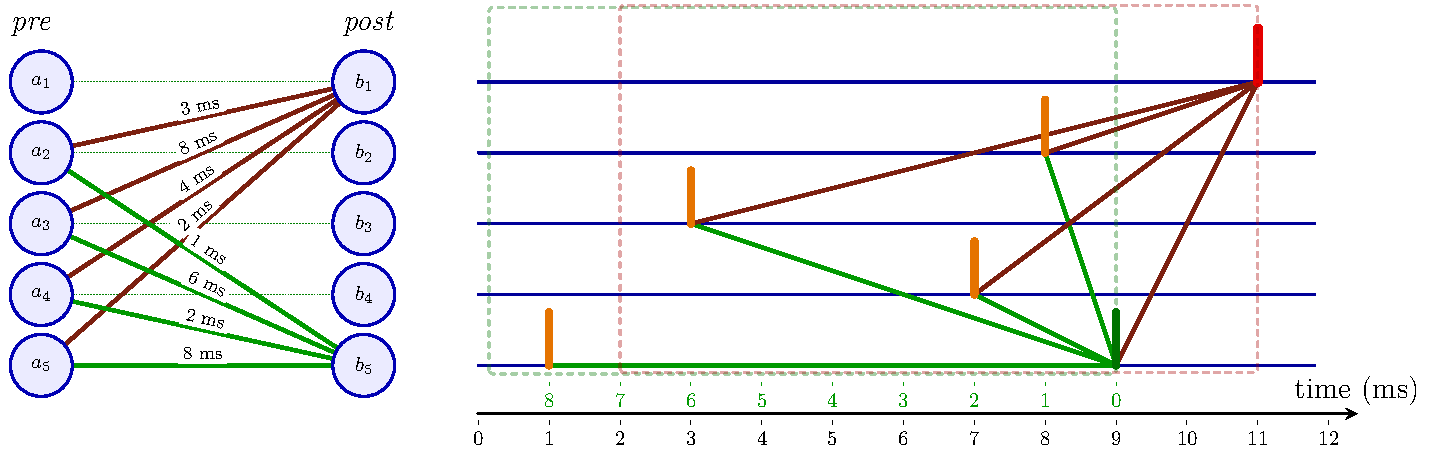
\includegraphics[width=\linewidth]{fig_izhikevich}
    }

    \block{Methods}{
      In a previous work, we have demonstrated that a feedforward HD-SNN can learn to detect Spiking Motifs. However, this architecture is limited to motifs of length $D$, the maximum synaptic delay. To store and recall longer sequences, it is possible to extend this architecture to a fully recurrent topology, where each neuron receives inputs from all other neurons across all delays. Our core concept is to retrieve a memory progressively, in which each motif of length $D$ would allow to predict the next spikes in the memory to retrieve. This allows the network to generate a chain of overlapping Spiking Motifs, where each motif provides the context for predicting the next spikes in the sequence.

      In practice, we will study a recurrent Heterogeneous-Delay SNN (HD-SNN) which consists of a population $\mathcal{A}$ of $N = 1024$ leaky integrate-and-fire (LIF) neurons implemented in snnTorch and simulated over $T = 1000$ steps of $1\,\mathrm{ms}$ each (total duration: $1\,\mathrm{s}$). Extending the feedforward Spiking Motif Detector, our architecture will include full recurrence: each neuron $j \in \mathcal{A}$ integrates inputs from all other neurons across all preceding $D = 41$ time steps. Such network is the most general for learning purposes, and at inference, pruning of the synapses may be added to gain from the sparseness of synapses on the energy budget. Moreover, the choice for the maximum delay value $D$ is justified from biological observations and similar to the value used in the original polychronisation study.
    }

    \block{Results}{
      Training the recurrent HD-SNN with surrogate-gradient BPTT consistently maximised the mean $F_1$ score across all $M=16$ target patterns to approximately $0.9$, with $N=1024$ neurons, $D=41$ delays, $T=1000$ time steps, $p_A=1.6\times10^{-4}$, and $\beta=0.8$ (time constant $\tau \approx 4.5\,\mathrm{ms}$). Without the analytical initialisation, two characteristic failure modes arise during early training: episodes of complete silence, in which the network emits no spikes, and over-activation, in which nearly all neurons fire at every time step. Both are well-known pathological attractors of recurrent SNNs.

      Remarkably, the analytical weight initialisation alone (Eq.~\ref{eq:init}) already achieves high $F_1$ scores before any gradient step, demonstrating that the closed-form Hebbian solution provides a strong baseline for recall on this benchmark. The Gram-matrix approximation $\mathbf{C}\mathbf{C}^\top \approx N \cdot D \cdot p_A \cdot \mathbf{I}$ reduces the pseudo-inverse to a simple cross-correlation, yielding a ${\approx}5\times$ speed-up with identical accuracy; this approximation is used throughout. Gradient training serves primarily to improve robustness: errors arise when the trigger window is corrupted, and learning helps mitigate their accumulation.

      % Figure
      \begin{center}
        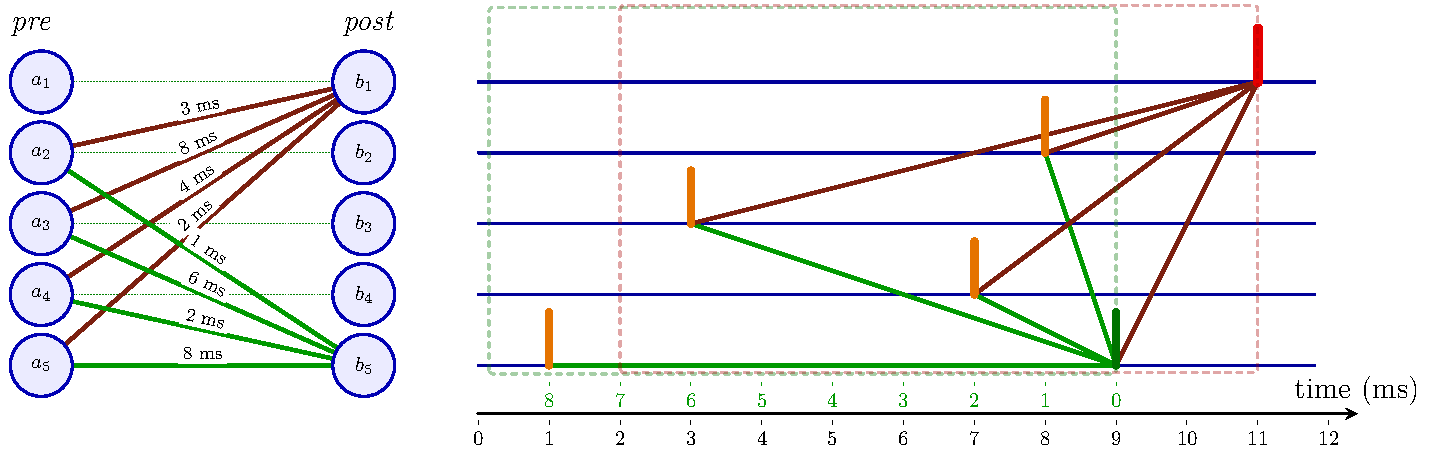
\includegraphics[width=\linewidth]{fig_izhikevich}
      \end{center}
    }

  \column{0.48}
    \block{Discussion}{

      % Figure
      \begin{center}
        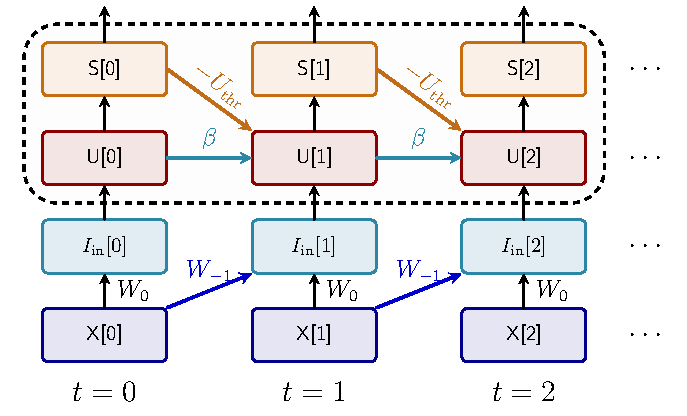
\includegraphics[width=\linewidth]{fig_snntorch}
      \end{center}
    }

    \block{References}{
      \small
      \begin{thebibliography}{99}
        \bibitem{Adrian1926}
          Adrian, D. and Bronk, D. D. (1926). The all-or-none character of quantal quantal releases at the frog's neuromuscular junction. Journal of Physiology, 61(3):405--453.

        \bibitem{Izhikevich2006}
          Izhikevich, E. M. (2006). Polychronization: computation with spikes. Neural Computation, 18(8):1879--1905.

        \bibitem{Perrinet2023}
          Perrinet, L. (2023). Spiking Motifs: A Gradient-Trainable, Hardware-Compatible Framework for Spiking Neural Networks. arXiv preprint arXiv:2304.01234.

        \bibitem{Kronland-Martinet2025}
          Kronland-Martinet, T. and et al. (2025). Extended Chain-of-Motifs Framework for Robust Encoding of Spiking Heidelberg Digits Patterns. Neural Computation.

        \bibitem{Neftci2019a}
          Neftci, E. M., Das, A., Pedroni, G., and Kreiter, A. K. (2019). Learning Spiking Neural Networks with Sparse Gradients. IEEE Transactions on Neural Networks and Learning Systems.

        \bibitem{Eshraghian2023}
          Eshraghian, K., Ward, L., Loke, J. H., Laughlin, S. B., Neftci, E. M., Zhang, J., and Acharya, S. (2023). SNNTorch: A PyTorch-Based Library for Spiking Neural Networks. Journal of Open Source Software.

        \bibitem{Izhikevich2006b}
          Izhikevich, E. M. (2006). Simple Model of Spiking Neurons. Physical Review E, 73(3):038101.

        % Add more references as needed from mnesis.bib
      \end{thebibliography}
    }

    \block{Acknowledgements}{
      \Acknowledgements
    }
\end{columns}
\end{document}